\documentclass[a4paper,11pt,oneside]{article}
\usepackage[T1]{fontenc}
\usepackage{ae,aecompl, textcomp, graphicx, xcolor, listings, float, url, amsmath, caption}
\usepackage[czech]{babel}
\usepackage[utf8]{inputenc}
\usepackage{csquotes}
\usepackage{fancyhdr}
\usepackage{indentfirst}

\usepackage{datetime}

\lstset{basicstyle=\ttfamily,
	showstringspaces=false,
	commentstyle=\color{red},
	keywordstyle=\color{RoyalBlue},
	literate=%
	{á}{{\'a}}1
	{í}{{\'i}}1
	{é}{{\'e}}1
	{ý}{{\'y}}1
	{ú}{{\'u}}1
	{ó}{{\'o}}1
	{ě}{{\v{e}}}1
	{š}{{\v{s}}}1
	{č}{{\v{c}}}1
	{ř}{{\v{r}}}1
	{ž}{{\v{z}}}1
	{ď}{{\v{d}}}1
	{ť}{{\v{t}}}1
	{ň}{{\v{n}}}1                
	{ů}{{\r{u}}}1
	{Á}{{\'A}}1
	{Í}{{\'I}}1
	{É}{{\'E}}1
	{Ý}{{\'Y}}1
	{Ú}{{\'U}}1
	{Ó}{{\'O}}1
	{Ě}{{\v{E}}}1
	{Š}{{\v{S}}}1
	{Č}{{\v{C}}}1
	{Ř}{{\v{R}}}1
	{Ž}{{\v{Z}}}1
	{Ď}{{\v{D}}}1
	{Ť}{{\v{T}}}1
	{Ň}{{\v{N}}}1                
	{Ů}{{\r{U}}}1 
}

\lstdefinelanguage{JavaScript}{
	keywords={break, case, catch, continue, debugger, default, delete, do, else, false, finally, for, function, if, in, instanceof, new, null, return, switch, this, throw, true, try, typeof, var, void, while, with},
	morecomment=[l]{//},
	morecomment=[s]{/*}{*/},
	morestring=[b]',
	morestring=[b]",
	ndkeywords={class, export, boolean, throw, implements, import, this},
	keywordstyle=\color{blue},
	ndkeywordstyle=\color{darkgray}\bfseries,
	identifierstyle=\color{black},
	commentstyle=\color{purple}\ttfamily,
	stringstyle=\color{red}\ttfamily,
	sensitive=true,
	tabsize=2,
	belowcaptionskip=0em
}

\DeclareCaptionFont{white}{\color{white}}
\DeclareCaptionFormat{listing}{\colorbox{gray}{\parbox{\textwidth}{~#3}}}
\captionsetup[lstlisting]{format=listing,labelfont=white,textfont=white}

\usepackage[DIV=14,BCOR=2mm,headinclude=true,footinclude=false]{typearea}
\PassOptionsToPackage{hyphens}{url}\usepackage{hyperref}

\setlength{\parindent}{4em}
\setlength{\parskip}{1em}
\renewcommand{\baselinestretch}{1.2}
\setlength{\parindent}{2em}

\newenvironment{noparskip}{
	\setlength{\parskip}{0em}
}

\begin{document}

\begin{titlepage}

\centering
{\scshape\large Wichterlovo gymnázium, Ostrava-Poruba,\\příspěvková organizace\par}
\vspace{1.2cm}

\includegraphics[width=0.18\textwidth]{../wigym}
\par
\vspace{2cm}
\vspace{1.5cm}
{\huge\bfseries Pokladní a fakturační systém\\multiplatformní aplikace\par}
\vspace{.3cm}
{\Large\itshape Tat Dat Duong\par}

\vfill
vedoucí práce\\
Mgr.~Lada \textsc{Stachovcová}
\vfill

% Bottom of the page
{\large \formatdate{13}{4}{2017}\par}
\pagebreak
\end{titlepage}

\pagenumbering{arabic}
\vspace*{\fill}
\vspace*{\fill}

\section*{Čestné prohlášení}

Prohlašuji, že jsem svou práci vypracoval samostatně, použil jsem pouze podklady (literatura, SW atd.) uvedené v~přiloženém seznamu a postup při zpracování a dalším nakládání je v~souladu se~zákonem č. 121/2000 Sb., o právu autorském, o právech souvisejících s~právem autorským a o~ změně některých zákonů (autorský zákon) v~platném znění.

\bigskip

\noindent Hlučín, \formatdate{13}{4}{2017}

\vspace*{\fill}

\pagebreak
\pagestyle{fancy}

\tableofcontents

\pagebreak
\section{Úvod}
Dne 13.~dubna 2016\cite{eetzakon} vešel v~platnost zákon o elektronické evidenci tržeb, zkráceně EET. S~tímto zákonem vyplývá povinnost podnikatele veškeré údaje o prodeji posílat online na systémy Finanční správy pro další vyhodnocení. Cílem tohoto zákona je omezit systematické krácení daňové povinnosti a zjednodušit daňové kontroly. Finanční správa si tímto zákonem slibuje větší přísun peněz do státního rozpočtu a vyrovnání podmínek na trhu. 

Podnikatelé, kteří doposud fungovali s klasickou \enquote{hloupou} kalkukačkou, jsou nuceni si s příchodem tohoto zákona obstarat novou pokladnu, která umí komunikovat se servery Finanční správy. 

Na trhu se po schválení zákona vyrojilo mnoho společností, od malých \enquote{start\-upů} až po velké telekomunikační firmy, kteří poskytují své vlastní EET řešení. Po podrobném přezkoumání nabídek dodavatelů jsem se rozhodl vytvořit svoji pokladnu pro vlastní účely. Motivací byla především cena a svoboda výběru hardwaru, kdy nejsem vázán na konkrétní přístroj či značku.

\section{Hardware}

Pro základní použití se musí pokladní zařízení skládat z~počítače, na kterém prodejce zadává zboží, a z tiskárny, která bude schopna tisknout účtenky pro zákazníka. Abych snížil náklady na minimum, rozhodl jsem se použít tablet jakožto \enquote{počítač} mé pokladny.

V rámci této práce jsem se pokusil vybavit 2 prodejny vyvinutým pokladním systémem. Majitelé první prodejny byli spokojeni s~klasickou kalkulačkou a usilovali o co nejnižší pořizovací náklady. Díky tomu, že již vlastnili jeden Android tablet, byl výběr hardwaru přímočarý. Stačilo jenom dokoupit Bluetooth termotiskárnu, kterou jsme s majitelem objednali z~Číny za necelých 800 Kč. Na tuzemském trhu by se taková tiskárna dala sehnat za 1 500~Kč.  

V druhé prodejně byly požadavky přísnější: byla vyžadována pokladna se schopností přepínat prodejce, otvírat pokladní zásuvky a zobrazovat ceny zakoupeného zboží na obrazovce pro zákazníka. Zároveň by systém měl podporovat vícero pokladen pro případné rozšiřování prodejny. S majiteli jsme zvolili obdobné řešení: tablet jakožto vstupní zařízení pro aplikaci. K tomu jsme dokoupili malý server, ke kterému je připojena tiskárna s pokladní zásuvkou a obrazovka. Díky serveru mohou prodejci používat vícero pokladen naráz a zároveň agregovat své tržby na jednom místě.

\begin{figure}[H]
	\centering
	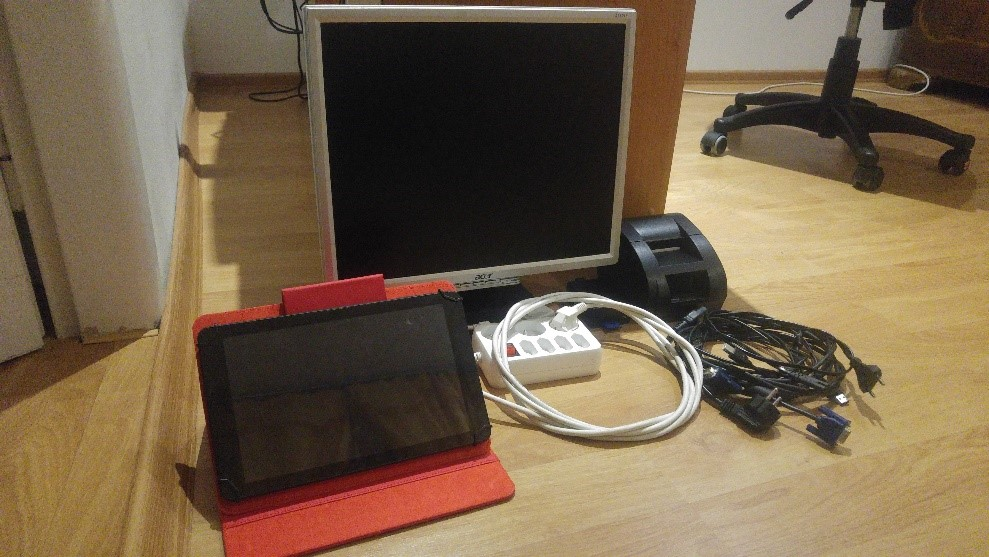
\includegraphics[width=0.7\linewidth]{../hardware}
	\caption{Hardware pro druhou prodejnu}
	\label{fig:hardware}
\end{figure}

\section{Struktura aplikace}
\label{sec:struktura}
Aplikace má strukturu klasické webové služby. Uživatel aplikaci vidí převážně jako webovou stránku, kterou si spustí na svém prohlížeči. Komunikaci se státní správou, tiskárnou a databází tržeb má na starost server. Pro Android jsem navíc vyvinul speciální prohlížeč pro pokladnu. 

\begin{figure}[H]
	\centering
	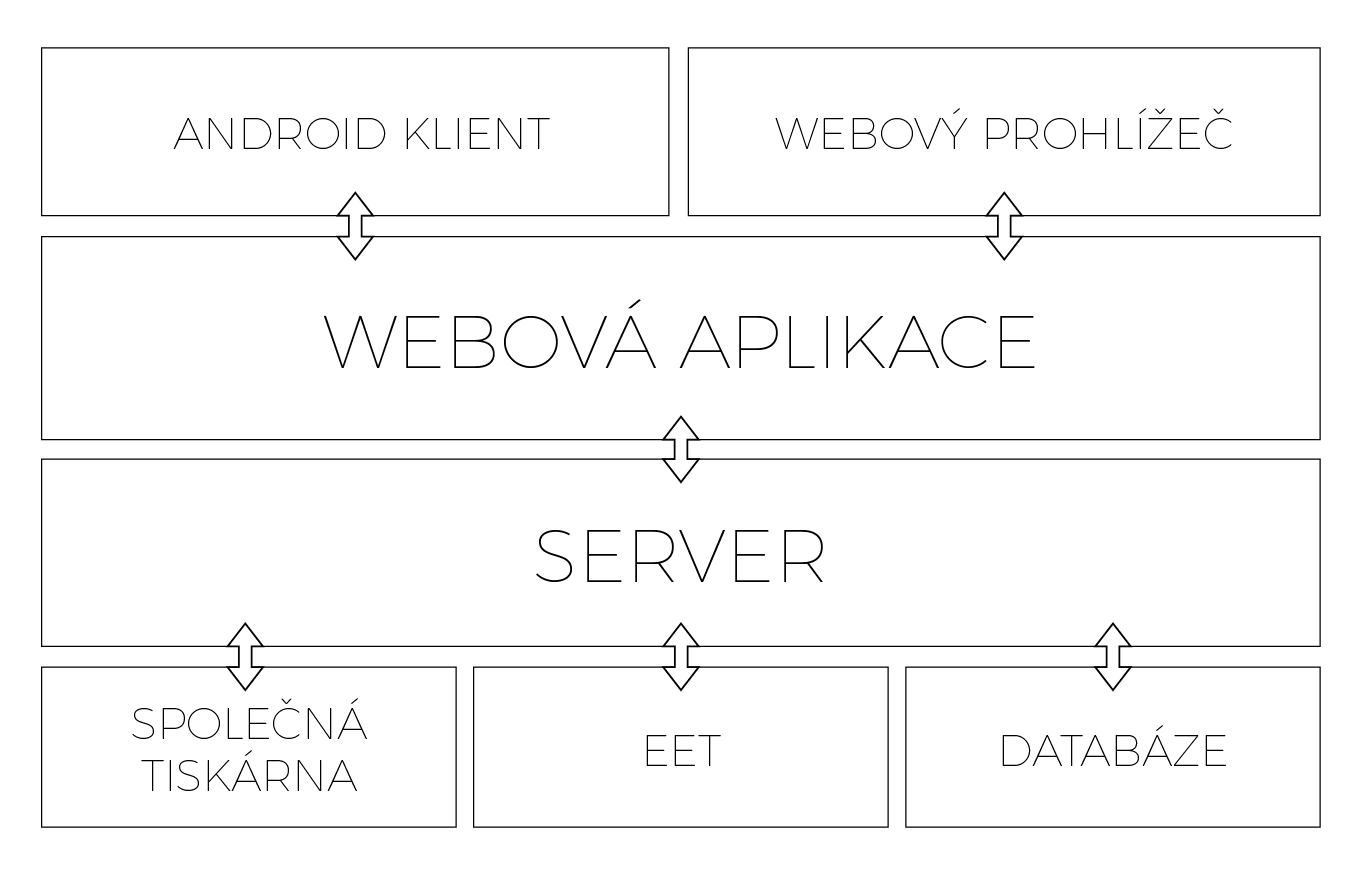
\includegraphics[width=0.65\linewidth]{../stack}
	\caption{Struktura aplikace}
	\label{fig:stack}
\end{figure}

Většinu kódu aplikace jsem napsal v~JavaScriptu. JavaScript je i přes své nevýhody \enquote{králem} multiplatformních jazyků. Jedná se totiž o jediný programovací jazyk, který může běžet jak v~prohlížeči, tak i samostatně na serveru.

\section{Technické specifikace}

Celá aplikace byla napsána v~JavaScriptu, přesněji ES2016. Zaměřil jsem se na psaní webové aplikace a jeho serveru, jelikož jsem neměl ponětí, na jakém přístroji aplikace poběží. S webovou aplikací mohou klienti aplikaci používat bez ohledu na platformu. Zároveň se tím vyhnu psaním nativních aplikací, což je jak na údržbu, tak na čas náročné. V~případě nutnosti je možné nativní aplikaci napsat, viz aplikace pro Android, která byla napsána v~Javě. 

Speciální zmínku si zaslouží velké all-in-one knihovny pro tvorbu mobilních aplikací jako Xamarin nebo Apple Cordova. Tyto frameworky mají své jisté nevýhody, a to v~jejich rozsáhlosti. Buď vyžadují vlastní jádro pro provoz (C\# a CLR) nebo se odkazují na knihovny, které by v~nemobilních zařízeních nefungovaly (Apache Cordova). V~konečném důsledku jsem se rozhodl psát v~čistém JavaScriptu.

Pro usnadnění vývoje (a vyzkoušení nových paradigmat) jsem použil následující knihovny:

\subsection{React}
\label{sec:react}

React je knihovna pro vytváření webových „komponentů,“ vyvíjena Facebookem. Laicky řečeno, pomocí Reactu vytváříme svoje vlastní HTML komponenty. Pro znalé, React by se dal chápat jako View část v~MVP architektuře (jako je Latte v~Nette). 

Obdobnou knihovnou ve sféře JavaScriptu je AngularJS. Spolu s~AngularJS patří mezi 2 nejpopulárnější frameworky pro vývoj UI. Oproti AngularJS má React plytčí křivku učení a syntax Reactu má k~čistému JavaScriptu blíže ve srovnání s~AngularJS.

Jak jsem jíž zmínil, účelem Reactu je psaní komponentů (dále už jen prvků). Tyto prvky různě vnořujeme a skládáme dohromady, až postupně dotvoří celou aplikaci. Psaní těchto komponent se řídí určitými pravidly a zásadami, které nám React ukládá jako povinnost. 

Základní myšlenkou Reactu je jednosměrnost dat. Místo toho, abychom psali kód, který volá příkazy a vykonává změny, píšeme kód, který pouze vykresluje aktuální stav aplikace. Řekneme prvku naše vstupní data a ten se podle těchto dat vykreslí. Neměl by přímo zasahovat do obsahu cizích prvků. Pokud bychom chtěli ten obsah prvku změnit, musíme změnit jeho vstupní data. Takhle zůstanou jednotlivé prvky izolovány.

\pagebreak
Typický zdrojový kód Reactu může vypadat takto:
\begin{lstlisting}[language=javascript, caption={JavaScript}]
import React from "react" //musíme nejprve importovat knihovnu React
class Ahoj extends React.Component {
	render() {
		return <div className="hello">Ahoj světe</div>
	}
}
//...
\end{lstlisting}

Nejedná se o chybu, HTML tagy jsou tady schválně. Jeden z~hlavních rysů Reactu je JSX, což je syntaktický cukr usnadňující zápis React prvků. Místo toho, abychom se učili složitý zápis Reactu, můžeme rovnou psát HTML kód. JSX transpilátor převede tento zápis tak, aby ho chápal i prohlížeč. 

Výsledek JSX transpilátoru:

\begin{lstlisting}[language=javascript, caption={JavaScript}]
import React from "react" //musíme nejprve importovat knihovnu React

class Ahoj extends React.Component {
	render() {
		return React.createElement("div", {className: "hello"}, 
		"Ahoj světe")
	}
}
\end{lstlisting}

Pro úplnost: nejedná se úplně o 1:1 klon HTML. JSX má své omezení plynoucí ze specifikací DOM a JS, kvůli kterých musíme psát atributy v~camelcase (místo \lstinline|class| píšeme \lstinline|className|).

Stejně jako v~DOMu, i React prvky se mohou do sebe vnořovat. Tady narážíme na první způsob, jakým způsobem předáváme prvku data. V~terminologii Reactu používáme tzv. \lstinline|props|. Předáváme prvku vstupní parametry.

\pagebreak
\begin{lstlisting}[language=javascript, caption={JavaScript}]
// ...
class Hlavní extends React.Component {
	render() {
		return <div>
		<Ahoj />
		<Jmeno name="David" surname="Duong" />
		<Pocitadlo />
		</div>
	}
}
\end{lstlisting}

\lstinline|<Ahoj />| je komponenta, kterou jsme si nadefinovali dříve. Jeho výstup bude vždy stejný (\enquote{Ahoj světe}). Jak jsme si již všimli, komponenta \lstinline|<Jmeno />| má dodatečné atributy, které dodávají prvku data. Ty můžeme v~kódu pro \lstinline|Jmeno| číst z~objektu \lstinline|props|. 

\begin{lstlisting}[language=javascript, caption={JavaScript}]
class Jmeno extends React.Component {
	render() {
		return <div>
		<h1>{this.props.name}</h1>
		<h2>{this.props.surname}</h2>
		</div>
	}
}
\end{lstlisting}

Pokud dojde ke změně parametrů (čili změní se nějaká hodnota v~\lstinline|props|), funkce \lstinline|render()| se s~novými daty znovu zavolá. O to se již React postará sám.  

\pagebreak
Zároveň si můžeme povšimnout, že mezi složenými závorkami můžeme psát znova JavaScript. Zápis mezi závorkami lze chápat jako zápis do hypotetické proměnné.

\begin{lstlisting}[language=javascript, caption={JavaScript}]
// OK zápisy
<div>{true}</div>                // let obsah = true 
<div>{foo ? true : false}</div>  // let obsah = foo ? true : false

// Nebude fungovat
<div>{if (foo) {}}</div>         // let obsah = if (foo) {}
\end{lstlisting}

Abychom uzavřeli kruh, můžeme nakonec mezi závorkami psát znova JSX. Často toto využívám v~kódu pro vykreslení vícero prvků v~cyklu.

\begin{lstlisting}[language=javascript, caption={JavaScript}]
let pole = [1,2,3]

// vytváříme pole divů
<div>{pole.map(prvek => <span>{prvek}</span>)}</div>  

// Výsledek je v~HTML výstupu ekvivalentní:
// <div>
//     <span>1</span>
//     <span>2</span>
//     <span>3</span>
// </div>
\end{lstlisting}

Kromě „props“ používáme i „state“ pro uchování stavu. Tam si uchováváme interní proměnné, kterými nemusíme zatěžovat celou aplikaci. Příkladem může být třeba skrytí detailů při kliknutí, nebo zaznamenání počtu kliků. 

\pagebreak
Interaktivitu zajišťujeme pomocí event atributů (události), jak jsme zvyklí z~JavaScriptu, (\lstinline|onClick()|, \lstinline|onSubmit()|…)\footnote{Abychom si uchovali k~dispozici přístup k~instanci, musíme předat this pomocí funkce \lstinline|bind()|. V~opačném případě dostaneme pouze DOM prvek, na kterém nastala událost.}. 

\begin{lstlisting}[language=javascript, caption={JavaScript}]
class Pocitadlo extends React.Component {
	constructor(props) {
		super(props)
		
		//inicializuje state, kdy ještě uživatel neklikl
		this.state = {kliknuti: 0}                                
	}
	
	kliknul() {
		// pro úpravu stavu musíme vždy volat 
		// this.setState(), který vyvolá vykreslení
		this.setState({kliknuti: this.state.kliknuti + 1})       
	}
	
	render() {
		<span onClick={this.kliknul.bind(this)}>
			{this.state.kliknuti}
		</span>
	}
}
\end{lstlisting}
\vspace*{\fill}
\pagebreak
\subsection{Redux}

Během čtení kapitoly \ref{sec:react} o Reactu Vás mohlo napadnout: \enquote{Odkud beru ta vstupní data a komu mám posílat změny v~datech?} Existuje mnoho způsobů, jak uchovávat všechna potřebná data jednotlivých prvků. Můžeme je uchovávat pro jednotlivé prvky zvlášť, což se ale ukázalo jako nepraktické a nepřehledné. Proto jsem přešel k~metodě \enquote{globální proměnné,} kde vše ukládám do~jednoho zdroje.

Pro zjednodušení práce s~globálním stavem používám knihovnu Redux, se kterou jsem napsal celou moji \enquote{business} logiku\footnote{Business logika -- kód, který reprezentuje model uživatele, tj. vše, co nemá na starost vykreslení a rozhraní}. Nejde však tak o knihovnu jako takovou, ale o zásady, které Redux doporučuje.

Na stránkách Reduxu můžeme najít, že s~Reduxem vytváříme „kontejner stavů.“ Musíme si nejprve vysvětlit, co vlastně stav aplikace je. Stav aplikace je podoba aplikace se všemi změnami v~určitém čase. Zahrnuje CSS třídy, HTML, ale i globální proměnné apod. V~běžné JavaScriptové aplikaci tento \enquote{aplikační stav} měníme několika způsoby:

\begin{itemize}
	\item změnou CSS tříd (\lstinline|document.queryElement("a").toggleClass("trida")|)
	\item změnou HTML obsahu: (\lstinline|document.queryElement("p").innerHTML = "obsah"|)
	\item změnou globálních promněných (\lstinline|window.localStorage.set("vnitřní proměnná")|)
\end{itemize}

Z toho důvodu se pak data nepředvídatelně mění na různých místech. Testování takovéto aplikace je složitější a pokryje většinou pouze uživatelské rozhraní. 

Použitím Redux zredukujeme počet zdrojů změn na jeden -- na jediný zdroj pravdy. Zdrojem této pravdy je tzv. \lstinline|kontejner|\footnote{V angličtině \lstinline|store|}. Tento zdroj obsahuje všechna data, které aplikace potřebuje pro svůj chod. Aplikace má číst svá data pouze z~toho kontejneru, nikde jinde. Z toho vyplývá, že stejná data musí uvést aplikaci vždy do stejného stavu. Pokud tedy máme předvídatelný stav, tak bude i aplikace předvídatelná a máme pod kontrolou celý chod aplikace.

Díky tomu je ladění a testování takové aplikace velice jednoduché, všechny změny pocházejí pouze z~jednoho zdroje. Stačilo mi pouze testovat samotný zdroj aplikace, v tomto případě jen jeden zdroj. 

\vspace*{\fill}
\pagebreak


Samotné testování je velice snadné. S Reduxem můžeme teoreticky testovat grafické rozhraní aplikace, aniž bychom testovali přímo v~prohlížeči. Zároveň implementace obtížných funkcí, jako je tlačítko \enquote{Vrátit zpět} či synchronizace aplikace napříč zařízeními, je díky tomuto přístupu mnohem snazší. 

Abychom se vyvarovali nepředvídatelným změnám, je v~aplikaci náš datový kontejner k~dispozici pouze pro čtení. Jediným způsobem, jak změnit naše data v~kontejneru, je pomocí \enquote{akcí.} Každá akce se musí skládat z~typu (co se má změnit) a popřípadě z~dat (jak se to má změnit). 

\begin{lstlisting}[language=javascript, caption={JavaScript}]
let action = (number) => {
	return { type: "set", number: number }
}
\end{lstlisting}

Samotné změny jsou prováděny pomocí \lstinline|reducerů|. Jsou to funkce, které vezmou předchozí stav, aplikují naši akci a vrátí stav nový. Nacházejí se vevnitř kontejneru a čekají, než odešleme nějakou akci.

Akci voláme do kontejneru pomocí \lstinline|store.dispatch(akce)|, který zavolá náš \lstinline|reducer|.

\begin{lstlisting}[language=javascript, caption={JavaScript}]
let initialState = 0 //počáteční stav, při inicializaci
let reducer = function(state = initialState, action) {
	if (action.type === "set") { //pokud máme akci 
		return action.number //vrátíme nový stav
	} 
	
	//další funkce
	
	return state // všechny akce provedeny, vrátíme nový stav
}
\end{lstlisting}

Abychom zachovali princip jediného zdroje pravdy, musí být jednotlivé stavy (výstupy z~reduceru) neměnné\footnote{V angličtině immutable}. To znamená, že nesmí existovat žádná metoda, která magicky změní data v~kontejneru, aniž by to prošlo přes \lstinline|store.dispatch()|. Pro primitivní datové typy (string, integer) toto nemusíme řešit, problém nastává u polí a objektů. Nelze jen slepě přiřadit nová data, musíme použít speciální syntax ES6, abychom zajistili neměnnost i u polí a objektů.

\pagebreak

\begin{lstlisting}[language=javascript, caption={JavaScript}]
//počáteční stav, při inicializaci
let initialState = {
	list: [],
	number: 0
} 

let reducer = function(state = initialState, action) {
	if (action.type === "set") {
		// vytváříme nový objekt a překopírujeme 
		// všechny prvky z předchozího stavu + aplikování akcí
		return Object.assign({}, state, { number: action.number })
	} else if (action.type === "add") { //vložení do pole 
		// spread operátor z ES6, vytváříme nové pole
		return Object.assign({}, state, { 
			list: [...state.list, action.number] 
		})
	} 
	return state // všechny akce provedeny, vrátíme nový stav
}
\end{lstlisting}

Celý kontejner nakonec vytvoříme pomocí funkce \lstinline|redux.createStore()|. Ta poskládá všechny naše reducery a postará se o to, aby při volání \lstinline|store.dispatch()| dostaly všechny reducery svoji akci. Změny v~datech kontejneru odposloucháváme přes \lstinline|store.subscribe()| a celý obsah kontejneru získáme voláním funkce \lstinline|store.getStore()|.

\begin{lstlisting}[language=javascript, caption={JavaScript}]
let store = redux.createStore(reducer)
store.subscribe(() => {
	console.log(store.getStore()) // Výsledek { list: [1], number: 5 }
})

store.dispatch(add(1))
store.dispatch(set(5))
\end{lstlisting}

Praktické využití knihovny najdete ve složce \lstinline|core/|.

\subsection{mDNS}

Pro uživatelskou přívětivost během instalace jsem chtěl přidat schopnost detekovat servery na síti, aniž by uživatel musel zadávat přesnou IP adresu a port serveru. Procházet celou lokální síť manuálně v~kódu je kvůli množství možných kombinací IP adres a portů téměř nereálné, proto jsem se rozhodl implementovat protokol mDNS\footnote{Multicast DNS}. Ten se hojně využívá v~IoT zařízeních a při sdílení obsahu na Wi-Fi síti. Příkladem může být Apple Bonjour a jeho AirPlay.

Pro provoz není třeba žádná konfigurace ze strany správce sítě. Stačí jenom mDNS službu spustit a klienti budou schopni automaticky získat IP adresu a port běžícího serveru. 

Prakticky je implementace mDNS vyřešena použitím knihovny \lstinline|resin-io/bonjour|, psána čistě v~JavaScriptu. Vyhneme se instalaci služby Avahi a kompilaci nativních knihoven. Díky tomu si můžeme být jistí, že je mDNS implementována na všech platformách stejně. 
Na straně Android klienta jsem musel importovat knihovnu \lstinline|jmDNS|. Obsahuje totiž novější implementaci mDNS protokolu oproti Android NSD\footnote{Network Service Discovery}. Často se nativní Android NSD zasekávala a pro obnovení funkčnosti byl vyžadován restart zařízení. 

Pro Android je zde ještě jedno zásadní omezení, a to ve formě IPv6. Chrome pro Android dosud stále nepodporuje IPv6 HTTP adresy. Problém nejspíš spočívá v~samotném Androidu, který v~době psaní této práce stále plně nepodporuje IPv6\cite{ipv6bug}. Z toho důvodu doporučuji vypnutí IPv6 na serveru.

U serverů běžících na Raspberry Pi je IPv6 vypnuto během instalace, manuálně lze IPv6 vypnout na systémech odvozených od Debianu vložením tohoto řádku do \lstinline|/etc/sysctl.conf|.

\begin{lstlisting}[language=bash, caption={sysctl.conf}]
net.ipv6.conf.all.disable_ipv6 = 1
\end{lstlisting}

\subsection{ESC/POS a tiskárny}

Většina termotiskáren využívá pro komunikaci protokol ESC/POS vyvinutý firmou EPSON. Tvoří jej sada textových příkazů, které se do tiskárny posílají. Každý příkaz tiskárny začíná znakem ESC (v ASCII kódování 27). Výjimku tvoří znak pro posun nového řádku, což je samozřejmě znak LF (ASCII = 10) a CR (ASCII = 13). Veškeré podporované příkazy lze najít v~souboru \lstinline|/server/printer/constants.js|. 

\pagebreak

Pro podporu češtiny je UTF-8 text překódován do Windows-1250/CP1250, jelikož většina tiskáren UTF-8 přímo nepodporuje. Samotná komunikace s~tiskárnou je řešeno otevřením souborového deskriptoru (FD) reprezentující tiskárnu, do kterého zapisujeme naše příkazy. Na Linuxu a Macu se FD otevře ve složce \lstinline|/dev/usb/lp[0-9]|. Ve Windows je nutné nejprve tiskárnu sdílet na síti. Posléze je k~dispozici na \lstinline|\\localhost\[název tiskárny]|.

Původně jsem s~tiskárnou přímo komunikoval za pomocí knihovny sériově, což se ukázalo jako velice nespolehlivé, obzvlášť pokud uživatel pravidelně vypíná tiskárnu po odchodu. Aplikace nebyla schopna znova nalézt tiskárnu a byl nutný restart celého systému. 

Tisk byl otestován na termotiskárnách dovezených z~Číny, konkrétně ZJ-5890K a ZJ-5805. Můžeme si být celkem jisti, že jsou podporovány všechny tiskárny, které umí protokol ESC/POS, což je na trhu většina.

\subsection{Linuxové aplikace v~Androidu}

Jak jsem již zmínil v kapitole \ref{sec:struktura}, aplikace se skládá z~webové aplikace a serverové části, kde většinu těžké práce vykonává server. Díky této architektuře jsme schopni provozovat více pokladen a agregovat data z~těchto pokladen na jednom místě. Problém nastane, když pokladnu potřebujeme jen jednu. 

Pro Windows, Linux a Mac je možné mít server a klienta na stejném zařízení. U mobilních platforem je provozování serveru problém. Obvykle se taková zařízení připojují na vzdálený server jako součást cloudové služby nebo mají serverovou část integrovanou v~klientovi. Provoz serveru na cloudu je však ekonomicky nevýhodný a integrace serverových části do klienta by znamenala možnou duplicitu kódu (serverová logika je na serveru i na klientu). Každopádně by obě řešení vyžadovala zásadní přepracování zdrojového kódu.

Naštěstí na pomoc přichází Termux\cite{termux}. Termux je open-source emulátor terminálu pro Android. Oproti ostatním emulátorům má Termux k~dispozici funkční příkaz apt-get a předkompilované Unix balíčky. Jedním z~těch předkompilovaných balíčků je i Node.JS, který pohání naši aplikaci na serveru. Rozhodl jsem se integrovat tento projekt do naší Android aplikace a využívat jejich repositáře.

Díky podpoře téměř všech klasických Linuxových aplikací jsme schopni aktualizovat aplikaci na pozadí, aniž bychom museli vydávat nové APK. Nezaznamenal jsem přitom žádný pokles výkonu během používání. Pouze je start aplikace znatelně pomalejší, což ve většině případů nedělá problém, jelikož většina obchodníků nechává zařízení neustále zapnuté. 

\pagebreak

Projekt Termux chráněn pod licencí GPL-3, proto bude zdrojový kód Android aplikace zveřejněn pod stejnou licencí. 


\subsection{Aktualizace a podpora}

Pro monitoring serveru používám aplikaci \lstinline|pm2|, která sleduje využití systémových prostředků a~v~případě pádu restartuje aplikaci. Vývojáři \lstinline|pm2| poskytují svoji placenou službu, která umožňuje sledovat logy a ovládat servery na dálku. Jelikož jedním z~cílů této práce bylo dosáhnout co nejnižší ceny, rozhodl jsem se vyvinout svoji vlastní alternativu postavenou nad \lstinline|pm2|. Server je napsán v~PHP. Díky tomu můžeme tento server provozovat za minimální cenu úplně kdekoliv.

\begin{figure}[H]
	\centering
	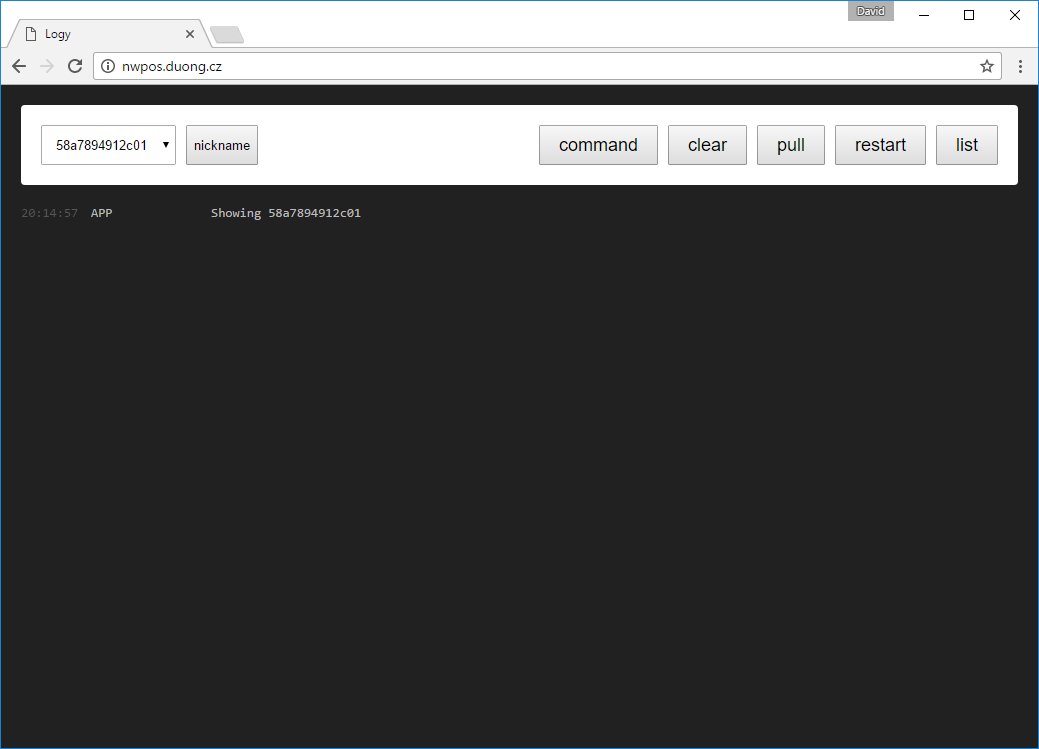
\includegraphics[width=0.5\linewidth]{../logs}
	\caption{Vývojářská konzole a výpis logů}
	\label{fig:logs}
\end{figure}

Pokladny pravidelně komunikují se serverem a odesílají svá data vygenerovaná při používání. Přes tuto aplikaci můžeme také odesílat příkazy pro restart či aktualizaci serveru. Díky tomu můžeme poskytovat podporu pro aplikaci i na dálku. Z bezpečnostních důvodů je tato funkce na pokladnách vypnutá, musí se manuálně spustit při prvotní instalaci.  

\pagebreak
\section{Instalace a provoz}
Dle požadavků prodejen, pro které jsem vyvíjel EET řešení, jsem vyvinul 2 způsoby, jakým lze provozovat tuto aplikaci. Z technického pohledu jsou řešeny identicky (viz kapitola \ref{sec:struktura}), liší se pouze ve způsobu instalace, který budu popisovat v~následujících kapitolách.

\subsection{Samostatný provoz}
\label{sec:samostatny}
Tento způsob je určen pro běžné uživatele, kteří se nechtějí zabývat složitou instalací a konfigurací. Stačí aplikaci nainstalovat a dle pokynů na obrazovce připojit veškeré příslušenství.

Pro Android poskytuji aplikaci, která nainstaluje veškeré závislosti a s~uživatelem projde nastavení pokladny. Před instalací bude nutné povolit \enquote{Instalaci z~neznámých zdrojů,} což lze učinit v~sekci \enquote{Nastavení \textrightarrow~Zabezpečení \textrightarrow~Neznámé zdroje} \eqref{fig:navodunknownsources}.

\begin{figure}[H]
	\centering
	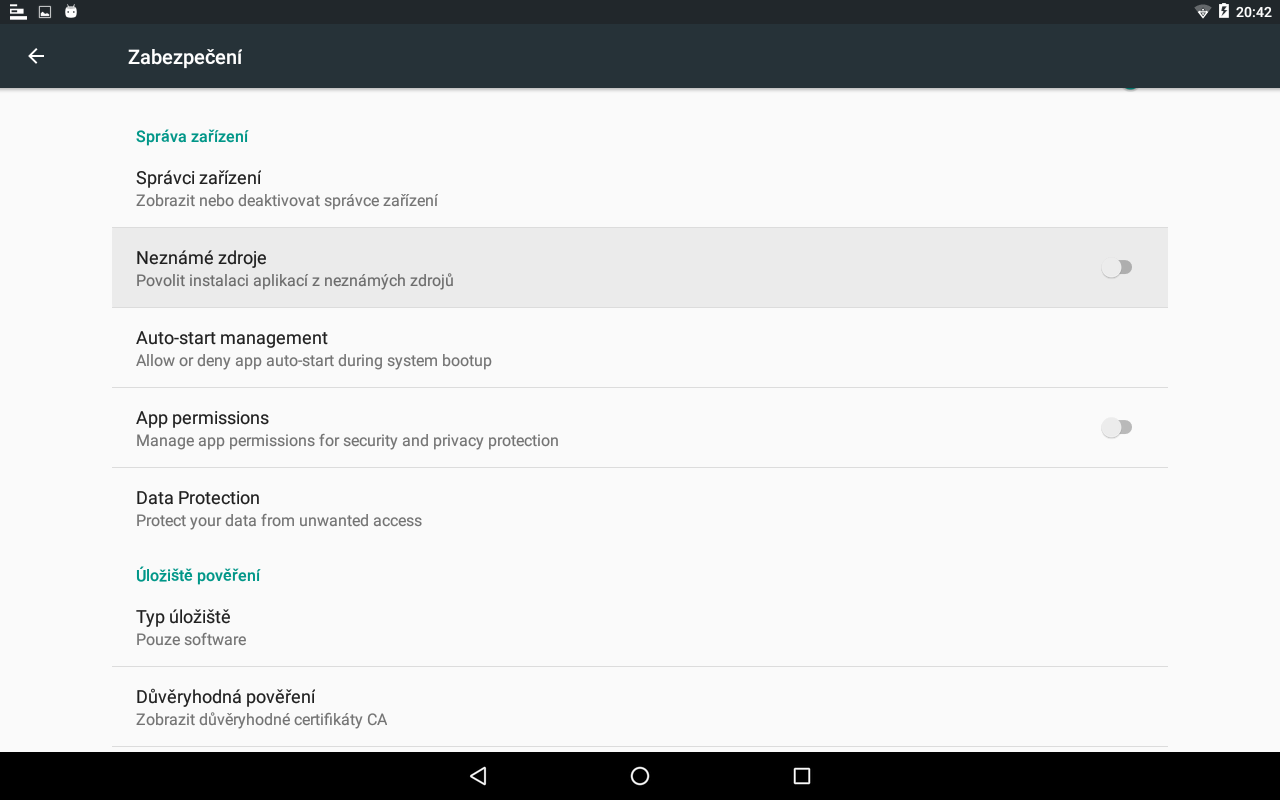
\includegraphics[width=0.6\linewidth]{../navod_unknown_sources}
	\caption{Neznámé zdroje}
	\label{fig:navodunknownsources}
\end{figure}

Po spuštění aplikace ze seznamu aplikací klikneme na tlačítko \enquote{Spustit bez serveru.} Aplikace začne stahovat potřebné knihovny pro běh bez serveru \eqref{fig:navodintro}.

\begin{figure}[H]
	\centering
	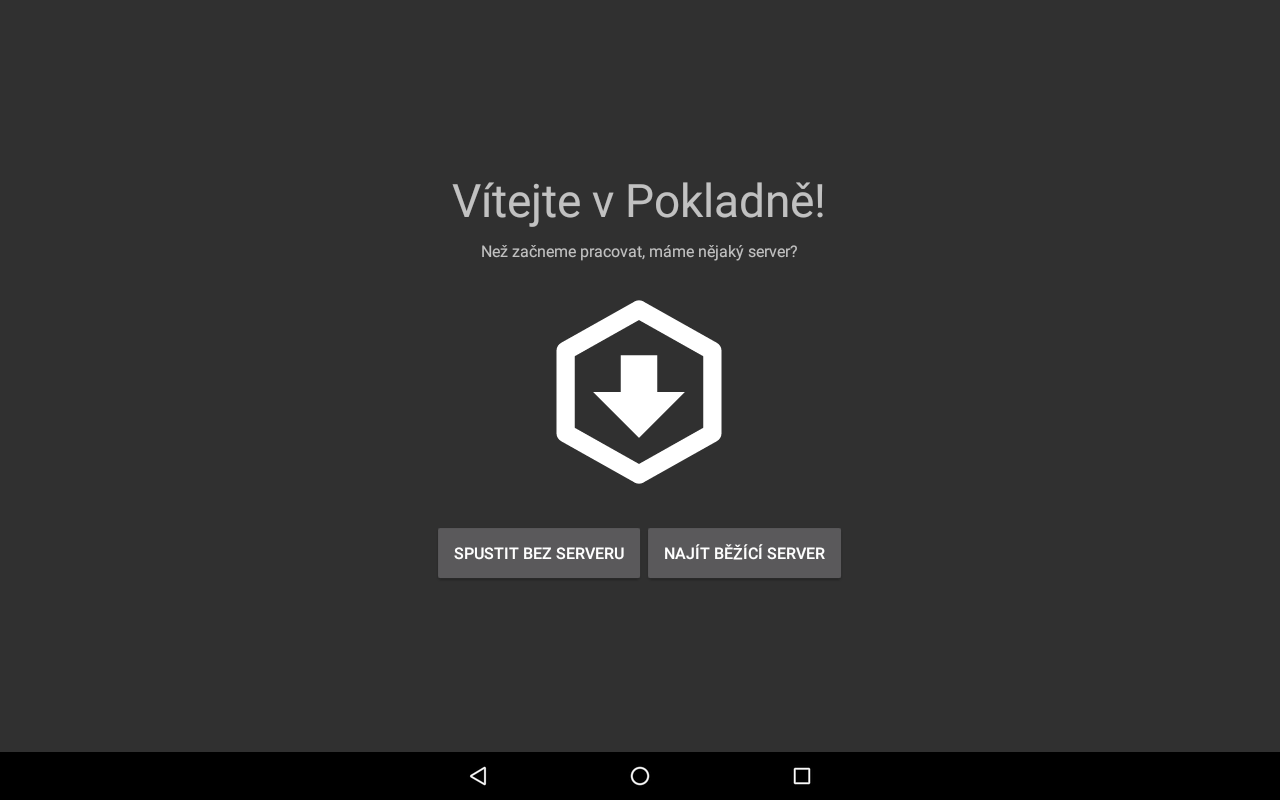
\includegraphics[width=0.6\linewidth]{../navod_intro}
	\caption{Úvodní obrazovka}
	\label{fig:navodintro}
\end{figure}

V další sekci se instalátor bude ptát na případnou Bluetooth tiskárnu, kterou bude zařízení používat. Instalaci dokončíme stisknutím na tlačítko \enquote{Přejít k~aplikaci} \eqref{fig:navodfinish}.

\begin{figure}[H]
	\centering
	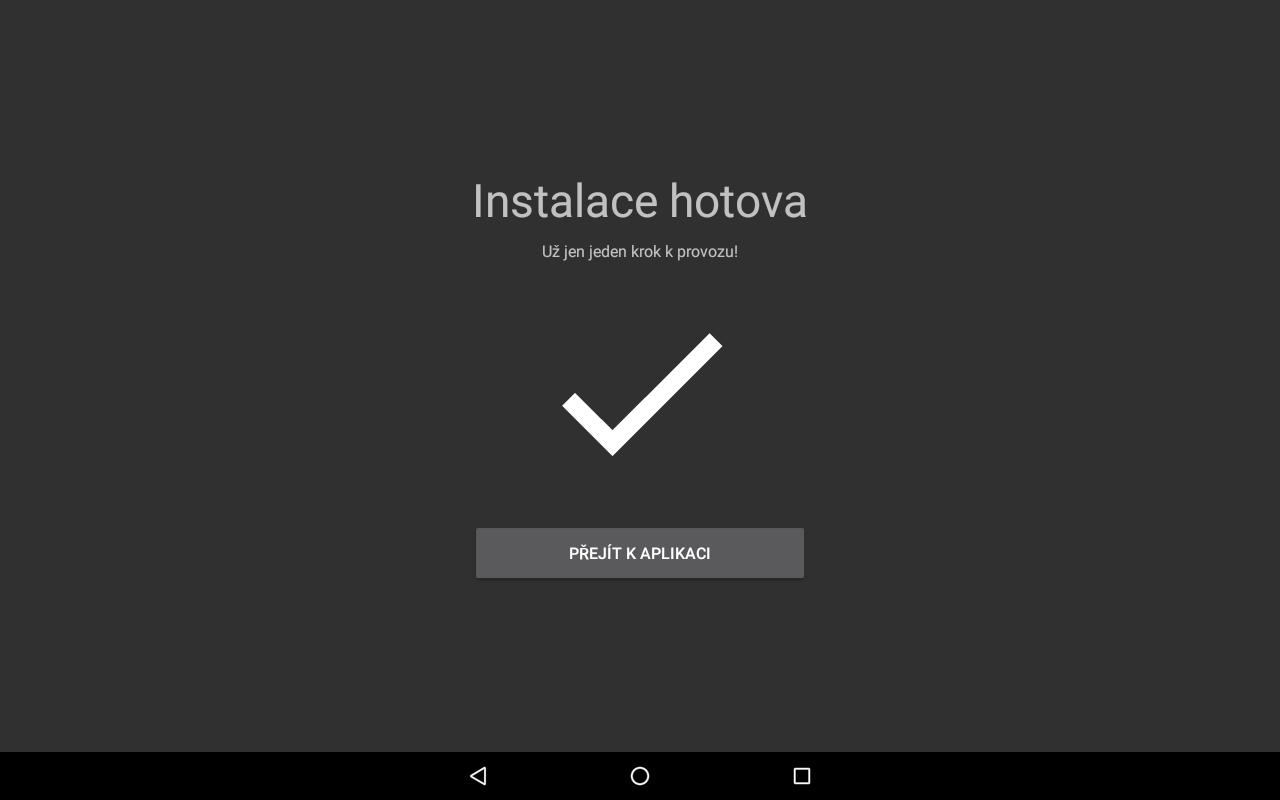
\includegraphics[width=0.6\linewidth]{../navod_finish}
	\caption{Instalace hotova}
	\label{fig:navodfinish}
\end{figure}

Po stisknutí tlačítka \enquote{Domů} se systém zeptá na výchozí spouštěč. Doporučuji nastavit \enquote{Pokladnu} jako výchozí spouštěč, čímž přepíšeme existující spouštěč a zabráníme zavření aplikace v~případě neúmyslného stisknutí \eqref{fig:uilauncher}.

\begin{figure}[H]
	\centering
	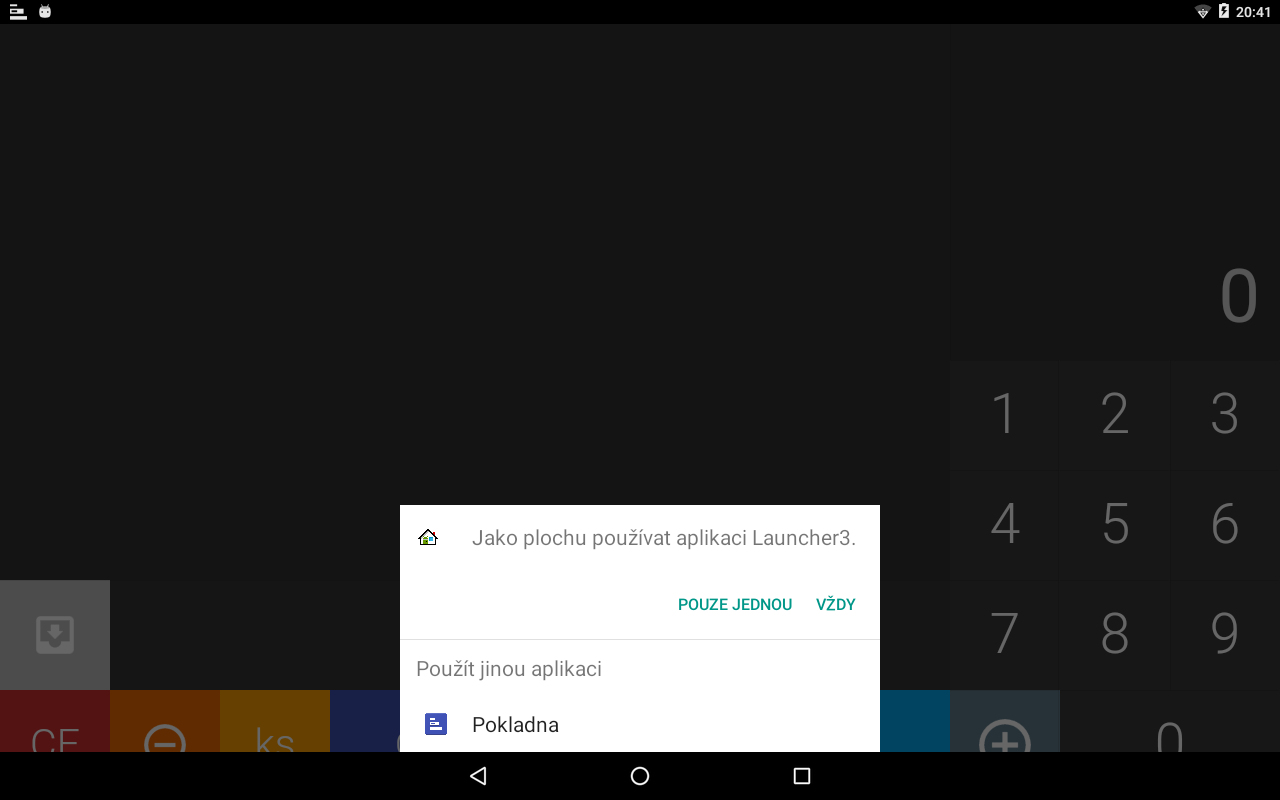
\includegraphics[width=0.6\linewidth]{../ui_launcher}
	\caption{Nastavení jako spouštěč}
	\label{fig:uilauncher}
\end{figure}

\subsection{Provoz \enquote{server a klient}}
Před instalací serverové aplikace je nutné nainstalovat a správně nakonfigurovat následující závislosti:

\begin{itemize}
	\item \lstinline|python2|
	\item \lstinline|nodejs| > 4.x
	\item \lstinline|python-pygame| -- pro zákaznický display
\end{itemize}
Instalace serveru je pak dokončena zadáním příkazu do příkazového řádku:

\begin{lstlisting}[language=bash, caption={Bash}]
$ npm install --production --prefix ./server
\end{lstlisting}

Po dokončení instalace se server spouští příkazem. Ve výchozím nastavení bude aplikace běžet na portu 8000. 

\begin{lstlisting}[language=bash, caption={Bash}]
$ node server
\end{lstlisting}

Aby se server spustil i po restartu počítače, je nutné nainstalovat službu, která bude monitorovat aplikaci a v~případě jejího pádu aplikaci restartovat. Pro monitoring jsem vybral odzkoušenou knihovnu \enquote{pm2.}

\begin{lstlisting}[language=bash, caption={Bash}]
$ sudo npm install -g pm2
$ sudo pm2 start ./server/ekosystem.json
$ sudo pm2 save
$ sudo pm2 startup
\end{lstlisting}

Pro Raspberry Pi máme připravený instalační skript, který nakonfiguruje počítač a nainstaluje veškeré závislosti. 

\begin{lstlisting}[language=bash, caption={Bash}]
$ sudo ./utils/config.sh
\end{lstlisting}

\subsubsection{Android}

Postup pro přidání pokladny k~serveru je obdobný jako u klasické samostatné instalace popsané v~kapitole \ref{sec:samostatny}. Po stažení a prvním spuštění aplikace klikněte na tlačítko \enquote{Mám vlastní server.} Aplikace se pokusí najít servery běžící na stejné síti. Vybranou síť pak zvolíte stisknutím na jméno serveru \eqref{fig:uidetectfound}. V~případě nutnosti lze adresu a port serveru zadat manuálně \eqref{fig:navoddetect}. 

Instalaci dokončíme stisknutím tlačítka \enquote{Přejít k~aplikaci} \eqref{fig:navodfinish}.

\begin{figure}[H]
	\centering
	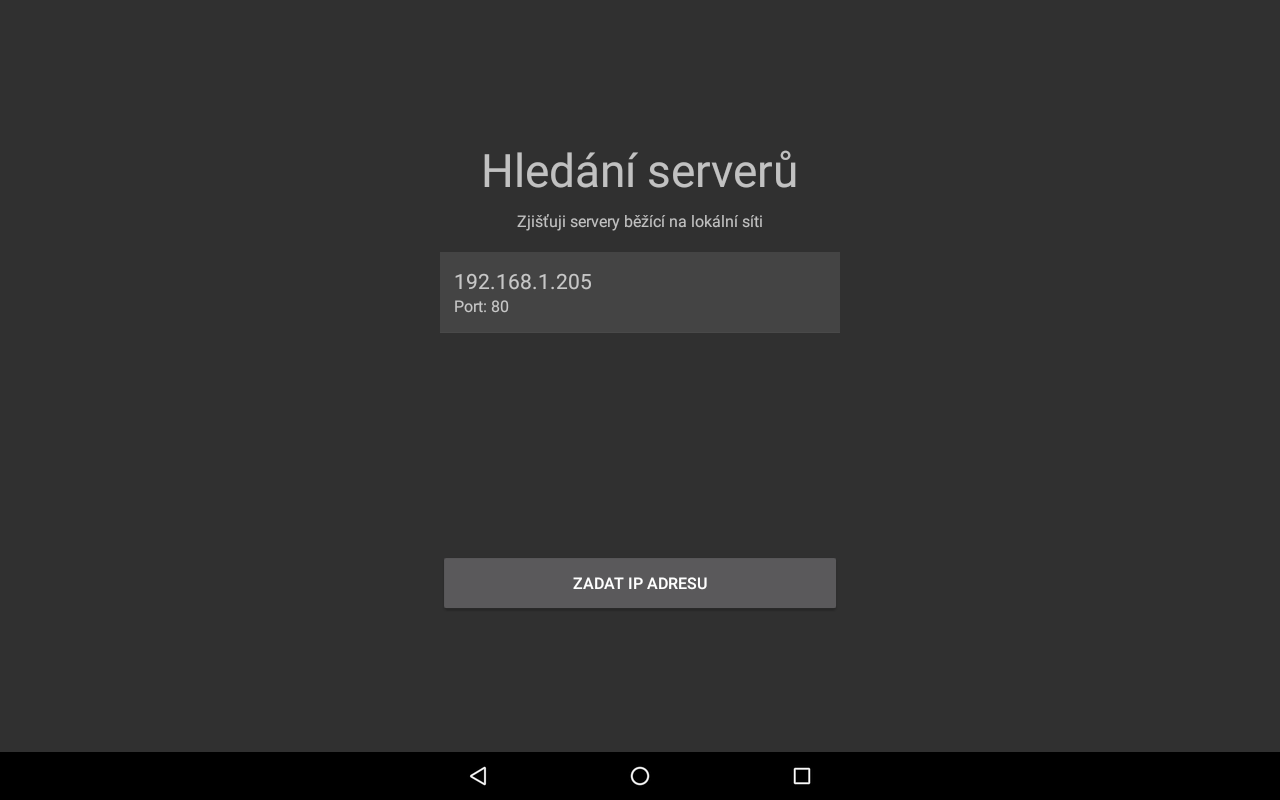
\includegraphics[width=0.6\linewidth]{../ui_detect_found}
	\caption{Výběr serveru ze seznamu}
	\label{fig:uidetectfound}
\end{figure}

\begin{figure}[H]
	\centering
	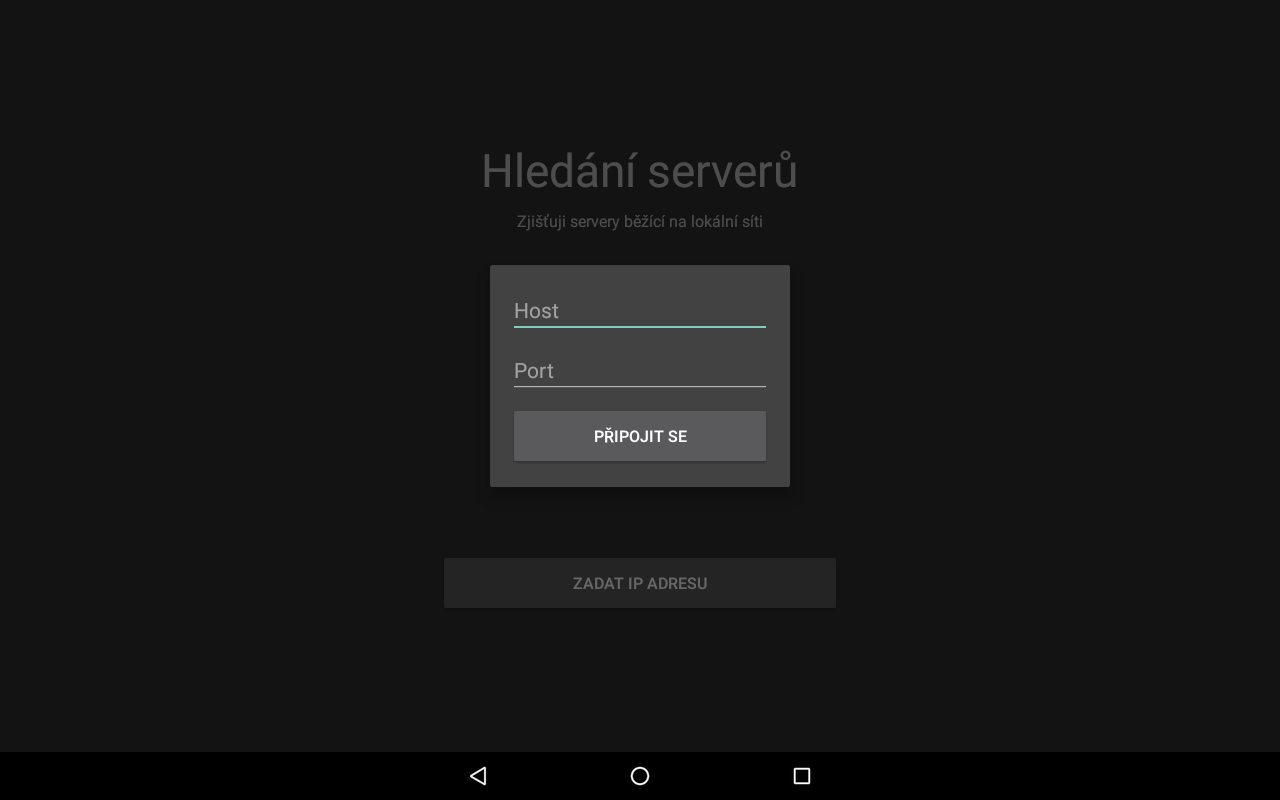
\includegraphics[width=0.6\linewidth]{../navod_detect}
	\caption{Zápis IP adresy a portu}
	\label{fig:navoddetect}
\end{figure}

\subsection{Návod k~použití}

Při prvotní instalaci budete požádáni o údaje provozovny. Ty jsou ukládány na straně serveru, tudíž po instalaci další pokladny tento krok nemusíte opakovat \eqref{fig:navodconfig}.

\begin{figure}[H]
	\centering
	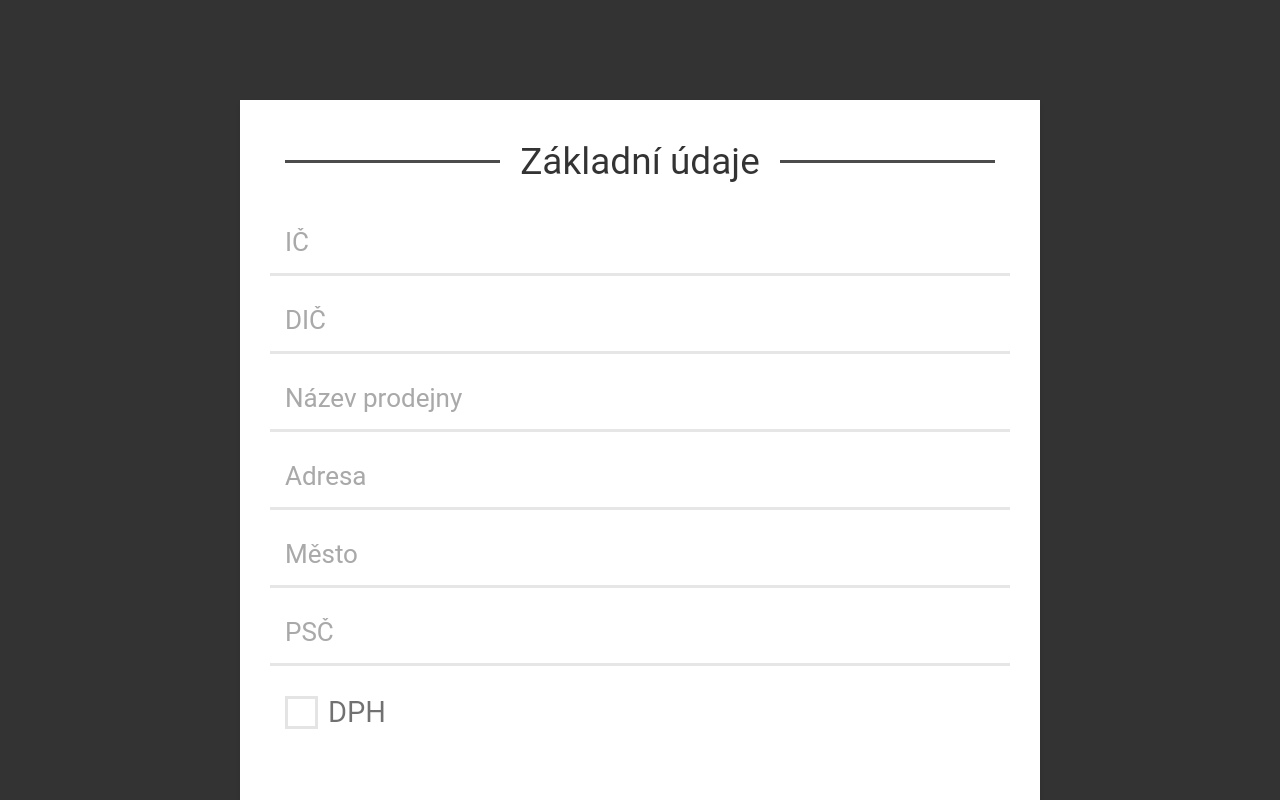
\includegraphics[width=0.7\linewidth]{../navod_config}
	\caption{Konfigurace provozovny}
	\label{fig:navodconfig}
\end{figure}


Po vyplnění a uložení můžete přejít do režimu pokladny. Aplikace je rozdělena na 2 panely. V pravém panelu uživatel zapisuje částky a vkládá je do košíku \eqref{fig:uipokladna}. 

\begin{figure}[H]
	\centering
	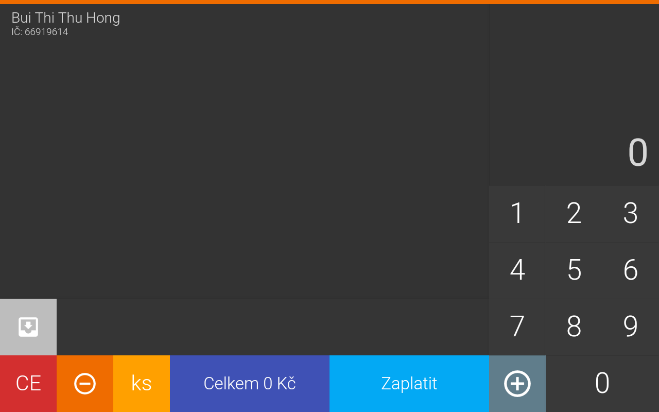
\includegraphics[width=0.7\linewidth]{../ui_pokladna}
	\caption{Rozhraní pokladny}
	\label{fig:uipokladna}
\end{figure}


Samotný košík se zobrazuje na levé části, kde můžeme upravit jednotlivé položky v~seznamu (změnit počet kusů, přejmenovat či smazat celou položku). Po kliknutí na název zboží se otevře vyskakovací okno s~možností editace názvu \eqref{fig:uikeyboard}.

\begin{figure}[H]
	\centering
	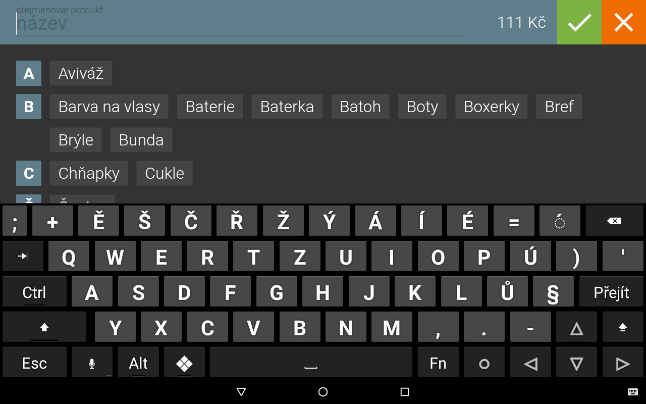
\includegraphics[width=0.7\linewidth]{../ui_keyboard}
	\caption{Přejmenování produktu}
	\label{fig:uikeyboard}
\end{figure}


Dole jsem umístil řídicí panel s~tlačítky pro smazání košíku, nastavení počtu kusů, přidání slevy, otevření pokladny nebo pro zadání platby, které slouží i jako přehled stavu košíku. Zároveň jsem implementoval našeptávač, který při psaní částky navrhuje možné názvy produktů vycházející ze statistik prodeje \eqref{fig:uisuggest}.

\begin{figure}[H]
	\centering
	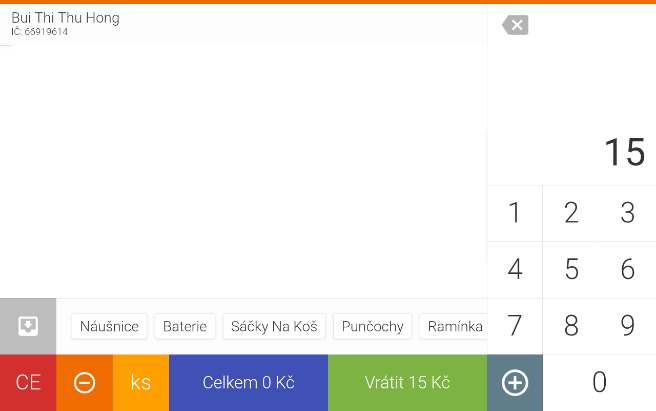
\includegraphics[width=0.7\linewidth]{../ui_suggest}
	\caption{Návrhy pro název zboží}
	\label{fig:uisuggest}
\end{figure}


Po rozbalení menu (v Androidu při přidržení tlačítka Zpět) můžeme přejít ke statistikám tržeb či nastavení vzhledu aplikace či provozovny \eqref{fig:uimenu}.

\begin{figure}[H]
	\centering
	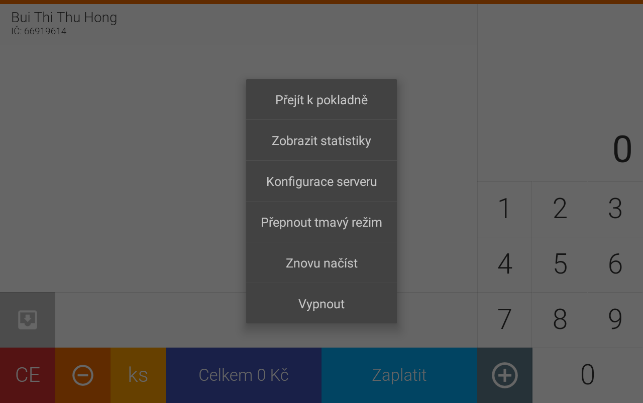
\includegraphics[width=0.7\linewidth]{../ui_menu}
	\caption{Menu aplikace (Android)}
	\label{fig:uimenu}
\end{figure}


Statistiky konkrétního dne si uživatel může rozkliknout po kliknutí na určitý den. V~případě potřeby je možné účtenku z~konkrétního dne znovu vytisknout. Smazání jsem pro účely evidence a kontroly s~FÚ neimplementoval \eqref{fig:uistats}.

\begin{figure}[H]
	\centering
	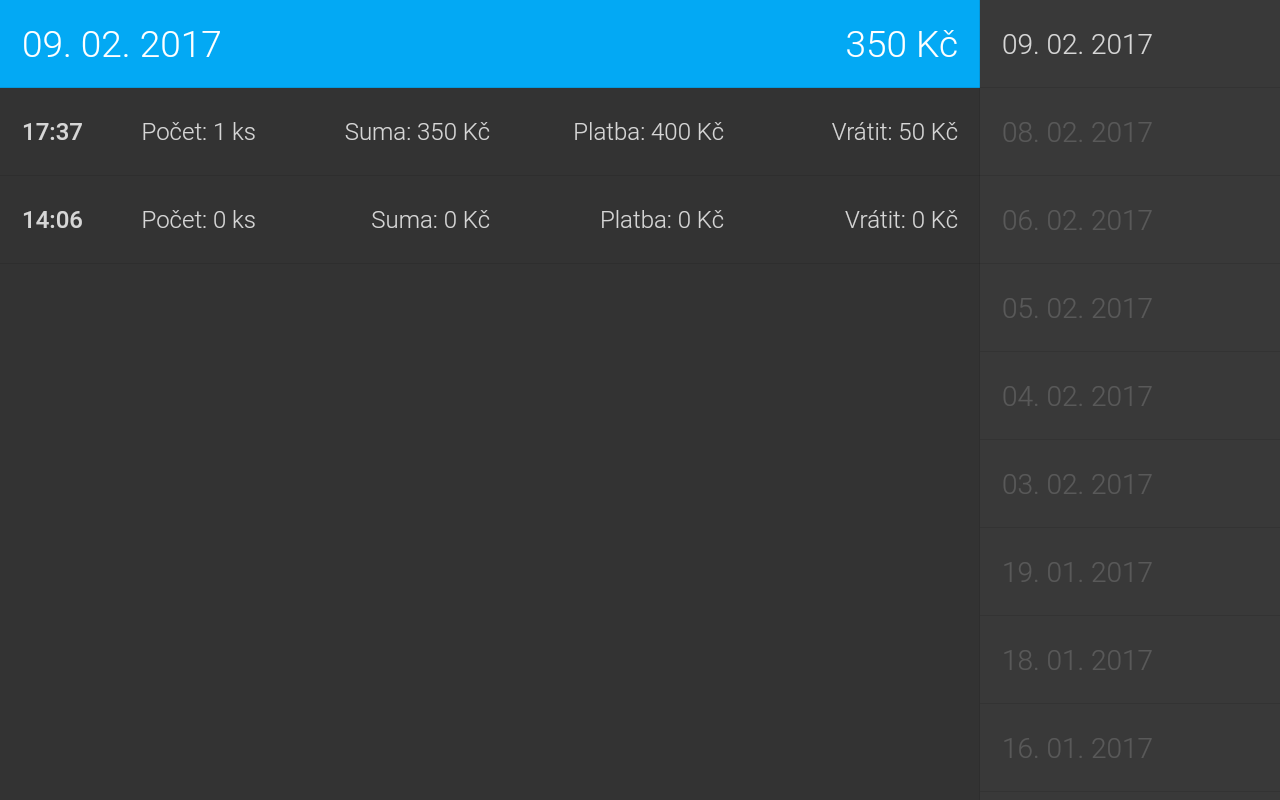
\includegraphics[width=0.7\linewidth]{../ui_stats}
	\caption{Statistiky prodeje}
	\label{fig:uistats}
\end{figure}

\pagebreak
\section{Závěr}
Vyvinul jsem dle zadání pokladní systém pro maloobchodní podniky. Oba podniky dnes spolehlivě fungují bez jakýchkoliv zádrhelů. Průměrná doba odesílání a získání FIK ze státní správy se stabilně pohybuje pod hranicí 1 sekundy i na slabších zařízeních díky ukládání WSDL do mezipaměti. Do budoucna bych chtěl aplikaci rozšířit o správu zboží, skladu a čtečku čárových kódů, což díky modularitě zdrojového kódu by neměl být problém.

Tento projekt byl zároveň produktem experimentování s~webovými technologiemi pro tvorbu aplikací jak pro mobil, tak pro klasický počítač. Web jakožto platforma pro jak mobilní, tak i~desktopové aplikace již není pouhým snem. Mnoho programátorů a firem dnes spoléhají na široké možnosti HTML, CSS a JS pro psaní prvotřídních aplikací určené pro milióny lidí. 

Výkonnostně jsou na tom nativní aplikace stále lépe. Sám jsem narazil na mnoho problémů s~rychlostí vykreslení a s odezvou. Postupnými úpravami a optimalizacemi jsem docílil srovnatelného výkonu jako u nativních aplikací, stále je zde ovšem velký prostor pro zlepšení. 

S příchodem WebAssembly, Service Workers a WebGL můžeme však s~jistotou očekávat, že budoucnost aplikací pro běžné uživatele bude jistě patřit webu. 

\pagebreak	
\begin{thebibliography}{Per00}
	\raggedright
	\bibitem{eetzakon} ČESKÁ REPUBLIKA. Zákon č. 112/2016 Sb. ze dne 13. dubna 2016 o evidenci tržeb. In: Sbírka zákonů České republiky. 2016, částka 43/2016. Dostupný také z: https://www.zakonyprolidi.cz/cs/2016-112.
	\bibitem{o2ekasa} PECHÁČKOVÁ, Lucie. eKasa vstoupila do ostrého provozu EET v roli lídra trhu. Tiskové centrum O2 Czech Republic [online]. 2016 [cit.~2017-04-03]. Dostupné z: https://www.o2.cz/spolecnost/tiskove-centrum/513034-eKasa\_vstoupila\_do\_ostreho\_provozu\_EET\_v\_roli\_lidra\_trhu.html
	\bibitem{ipv6bug} Support for DHCPv6 (RFC 3315): Android Open Source Project - Issue Tracker [online]. 2014 [cit. 2017-04-03]. Dostupné z: https://code.google.com/p/android/issues/detail?id=32621
	\bibitem{termux} FORNWALL, Fredrik. Termux: Android terminal emulator and Linux environment. [software]. GitHub, 2017 [cit. 2017-04-03]. Dostupné z: https://github.com/termux/termux-app
\end{thebibliography}

\pagebreak

\begin{noparskip}
	\listoffigures
\end{noparskip}


\section*{Seznam příloh}

\begin{itemize}
	\item DVD se zdrojovým kódem, dokumentací v~.pdf a .tex
\end{itemize}


\end{document}
